\chapter{Il processore}
Si descriver\`a la struttura di un processore facendo riferimento a un set di istruzioni ridotto: accesso a memoria, aritmetico logiche e di salto. Le prime due fasi
dell'esecuzione sono comuni a tutte le istruzioni e sono:
\begin{itemize}
\item Prelievo dell'istruzione da memoria.
\item Lettura del valore di uno o pi\`u registri operandi estratti direttamente dai campi dell'istruzione. 
\end{itemize}
Gli altri passi sono simili: tutte le istruzioni a parte quella di jump incondizionato utilizzano la ALU dopo aver letto gli operandi, o per calcolare l'indirizzo nel
caso di istruzioni di accesso a memoria, il calcolo del risultato nel caso di operazioni logico-aritmetiche o per il calcolo del confronto nel caso delle operazioni di 
salto condizionato. Dopo l'utilizzo dell'ALU le operazioni si differenziano: le istruzioni di accesso a memoria richiedono o salvano il dato in memoria, le operazioni
logico aritmetiche salvano il risultato nel registro target, le operazioni di salto condizionato cambiano il valore del program counter. 
\begin{figure}
  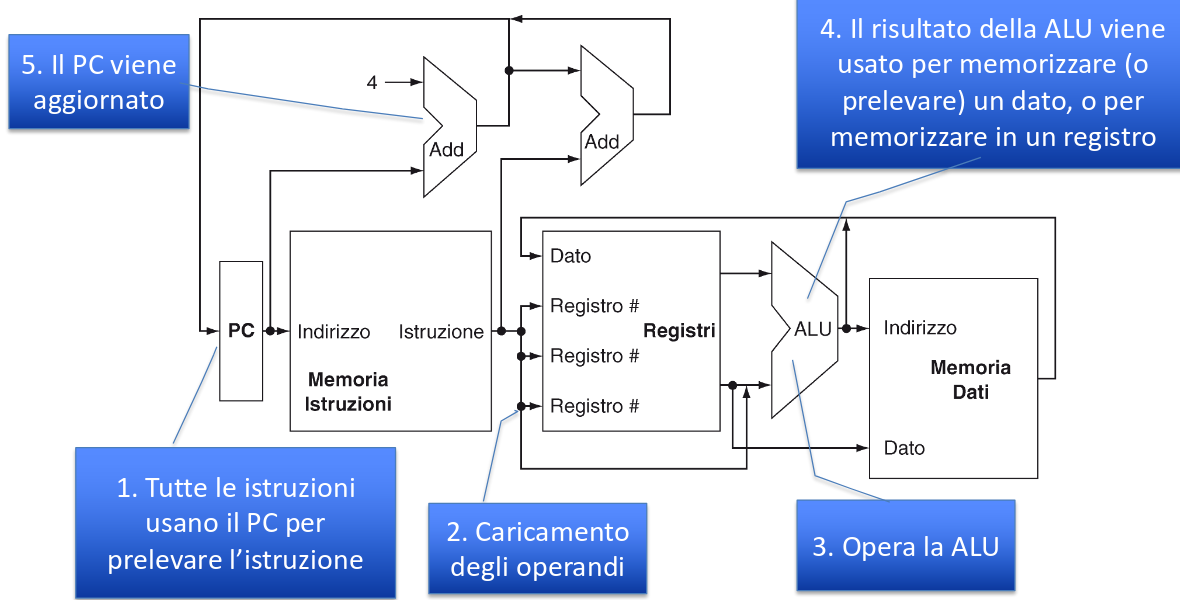
\includegraphics[scale=0.2]{Pictures/CPUBase.png}
  \caption{Un processore base}
  \label{fig:boat1}
\end{figure}
\newpage
La figura precedente \`e incompleta in quanto i dati arrivano da diverse sorgenti dalle quali bisogna scegliere, come per esempio per l'incremento del PC o la differenza
tra istruzioni di tipo R o di tipo I, in cui un dato pu\`o provenire da un registro o essere contenuto nell'istruzione. Per selezionare quale delle operazioni svolgere
viene utilizzato un multiplexer, che sulla base di un ingresso di controllo sceglie quale degli input debba finire in un output. Le linee di controllo del multiplexer 
vengono impostate sulla base del tipo di istruzioni. I vari gruppi funzionali hanno ulteriori ingressi di controllo: la ALU per decidere quale operazione effettuare, il
banco registri ha un ingresso per decidere se scrivere in un ingresso o meno, la memoria dati ha degli ingressi per decidere se si vuole svolgere un'operazione di lettura
o scrittura. La decisione dell'impiego degli ingressi di controllo \`e associata ad un'ulteriore unit\`a funzionale.
\begin{figure}
  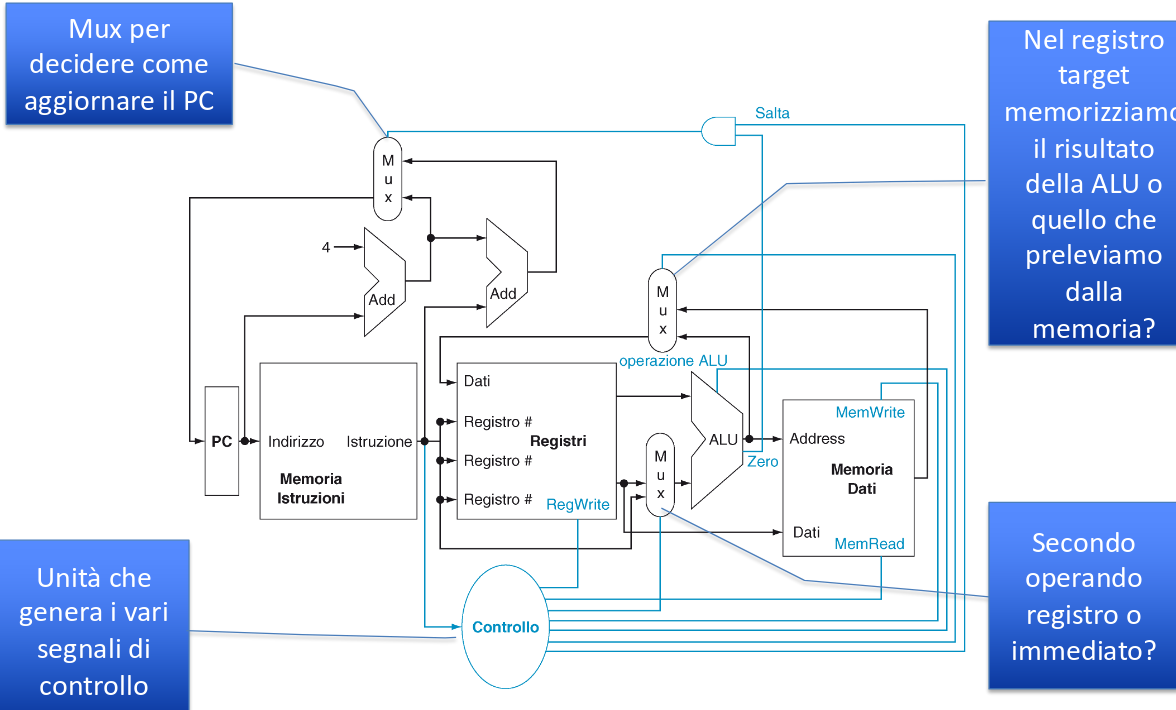
\includegraphics[scale=0.2]{Pictures/CPUDettagliata.png}
  \caption{Un processore pi\`u dettagliato}
  \label{fig:boat1}
\end{figure}
\newpage
Si pu\`o fare un'assunzione semplificativa dicendo che il processore lavora sincronizzandosi con i cicli di clock, e si assuma inoltre che tutte le operazioni si svolgano
in un unico ciclo abbastanza lungo. 
\section{Temporizzazione}
Questa metodologia esplicita quando i segnali possono essere letti o scritti in relazione al clock. Quella pi\`u utilizzata \`e quella sensibile ai fronti, in cui il dato 
viene memorizzato in corrispondenza della salita o della discesa del fronte di clock. I dati presi dagli elementi di stato sono relativi al ciclo precedente. Il tempo 
di clock deve essere scelto in modo da permettere ai dati di attraversare la rete combinatoria. Questa metodologia permette di rendere determinate operazioni che senza
di essa sarebbero indecidibili. 
\section{realizzazione del datapath}
Si passino in rassegna le componenti necessarie per realizzare un datapath:
\begin{itemize}
\item Una memoria istruzioni, dove sono salvate le istruzioni da eseguire.
\item Il program counter, l'indirizzo dell'istruzione da eseguire.
\item Il sommatore, un ALU specializzata a incrementare il PC. 
\end{itemize}
Questi elementi permettono il prelievo dell'istruzione:
\newpage
\begin{figure}
  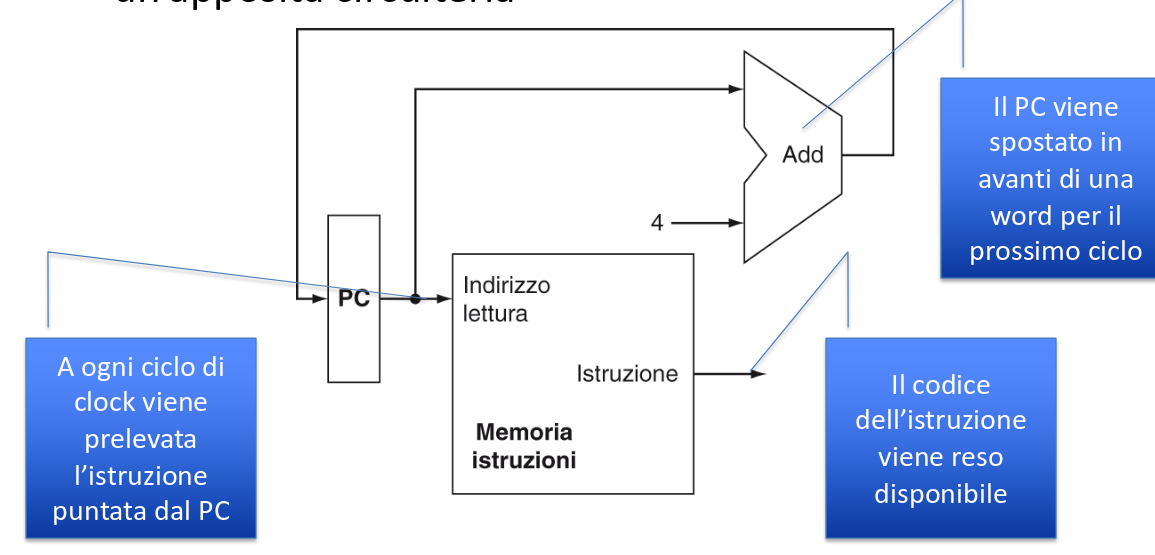
\includegraphics[scale=0.2]{Pictures/PrelievoIstruzione.png}
  \caption{Il processo di prelievo di un'istruzione}
  \label{fig:boat1}
\end{figure}
\subsection{Istruzioni di tipo R}
Le operazioni di tipo R sono istruzioni aritmetico-logiche che operano tra registri e producono un risultato in un altro registro. Per operare queste operazioni si
necessita di altri due blocchi funzionali:
\begin{itemize}
\item Il banco registri, che d\`a in output i registri specificati dell'istruzione e se abilitato in scrittura (regWrite) 0da un multiplexer scrive nel registro 
specificato il dato in ingresso.
\item Una ALU che effettua l'operazione specificata da una codifica a 4 bit, setta un bit in uscita se il risultato \`e zero.
\end{itemize}
\subsection{Istruzioni load store}
Per entrambe si deve calcolare un indirizzo di memoria dato dalla somma di un registro con un offset e nel caso di un'operazione di scrittura leggere il registro dal 
register file. Si necessiter\`a ancora pertanto di ALU e register file. Si noti che essendo l'offset memorizzato in un campo a 16 bit occorrer\`a un'unit\`a funzionale
in grado di estendere il segno a 32 bit. Dovr\`a essere inoltre essere aggiunta un'unit\`a di memoria dati da dove leggere e salvare i dati. Verr\`a utilizzata in 
scrittora (MemWrite) o in lettura (MemRead) in base al segnale dato dall'apposito multiplexer. 
\subsection{Salto condizionato}
Per compiere un salto condizionato si necessita di sommare un offset che dovr\`a essere esteso a 32 bit al PC. Siccome quest ultimo verr\`a sempre automaticamente 
aumentato di 4 verr\`a aggiunto al PC gi\`a aumentato. L'offset inoltre viene automaticamente traslato di due bit in modo da esprimerlo come word e non come byte e 
estendento cos\`i l'intervallo degli offset raggiungibile. Occorre pertanto un ulteriore multiplexer che decida se operare sul PC un'operazione di Pc+4 o PC+4+offset.
Per il salto incondizionato basta sostituire il campo offset shiftato di 4 al PC.
\begin{figure}
  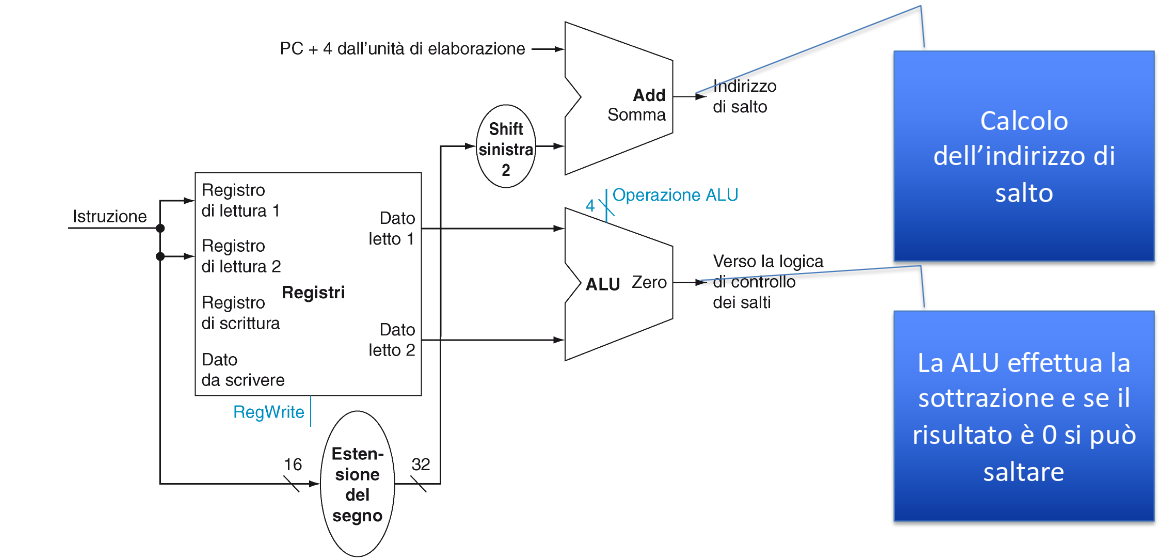
\includegraphics[scale=0.2]{Pictures/SaltoCondizionato.png}
  \caption{Il processo di Salto Condizionato}
  \label{fig:boat1}
\end{figure}
\subsection{Progetto di un'unit\`a di elaborazione}
Siccome ogni unit\`a funzionale pu\`o essere utilizzata un'unica volta per ogni ciclo di clock, si necessiter\`a di distinguere tra memoria dati e memoria istruzioni. 
Occorre inoltre condividere il pi\`u possibile le varie unit\`a. 
\newpage
\begin{figure}
  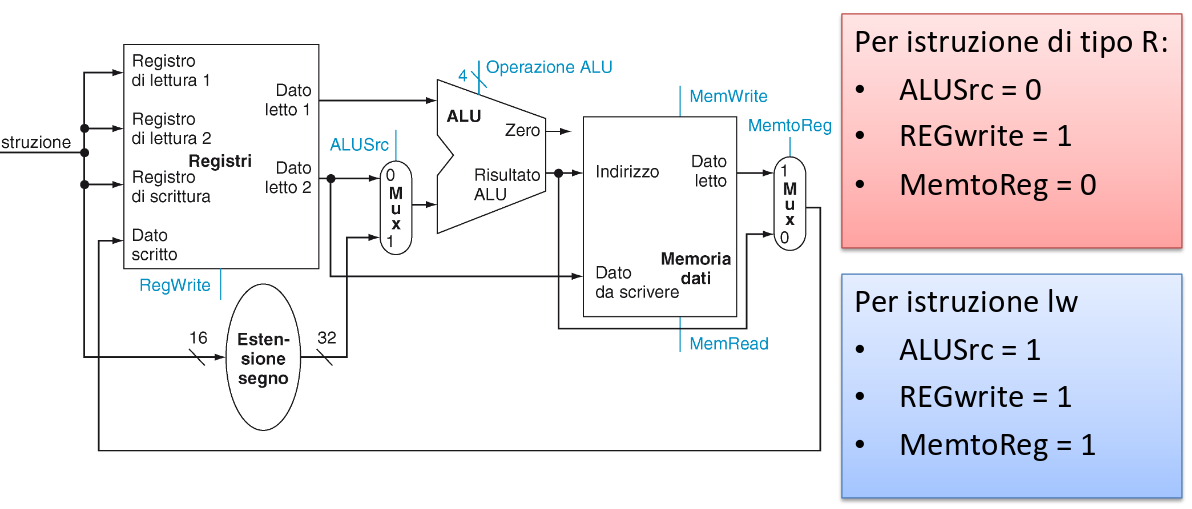
\includegraphics[scale=0.2]{Pictures/RMemoria.png}
  \caption{Circuito per istruzioni R e di trasferimento in memoria}
  \label{fig:boat1}
\end{figure}
\begin{figure}
  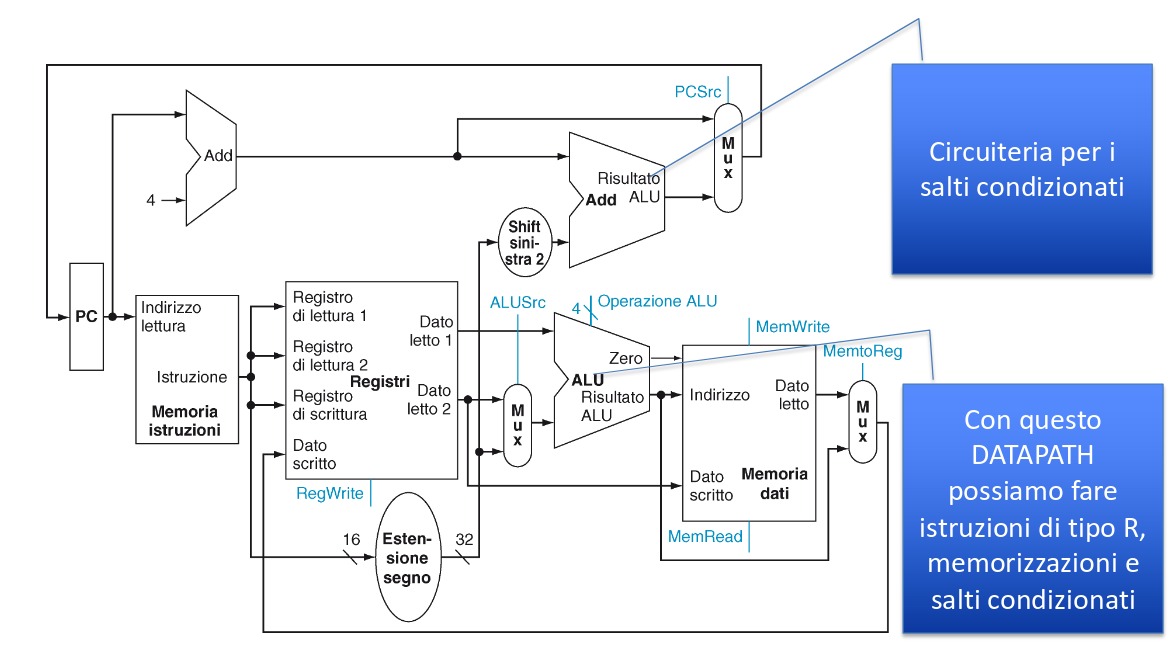
\includegraphics[scale=0.2]{Pictures/RMemoriaCompleto.png}
  \caption{Circuito per istruzioni R e di trasferimento in memoria dettagliato}
  \label{fig:boat1}
\end{figure}
\subsection{Prima implementazione comleta}
Per arrivare a una prima implementazione completa si parta dal datapath mostrato e si aggiunga la parte di controllo, implementando le istruzioni add, sub, and, or, slt, 
lw, sw, beq e successivamente il jump. 
\subsubsection{ALU}
La ALU viene utilizzata per realizzare operazioni logico aritmentiche di tipo R e slt, calcolare indirizzi di memoria e la sottrazione per beq. Per queste operazioni si
ha una diversa configurazione degli input di controllo (a 4 bit), si veda la tabella sulle slide. Per generarli si utilizza un'unit\`a di controllo che prende in 
ingresso il campo funct prelevato dall'istruzuione e due bit detti ALUop, ovvero 00 per sw e lw, 01 per beq, 10 per operazioni di tipo R specificate dal funct. Si genera
pertanto un comando attraverso due livelli: il primo genera i segnali di controllo ALUop per l'unit\`a di controllo della ALU, il secondo genera i segnali di controllo
per la ALU. I segnali di controllo della ALU sono generati da una rete logica combinatoria e per evitare di elencare tutte le combinazioni di ingresso ALUop e dei campi
funct vengono compressi attraverso l'utilizzo della wildcard X. Si vedano le tabelle delle slides.
\newpage
 \begin{figure}
  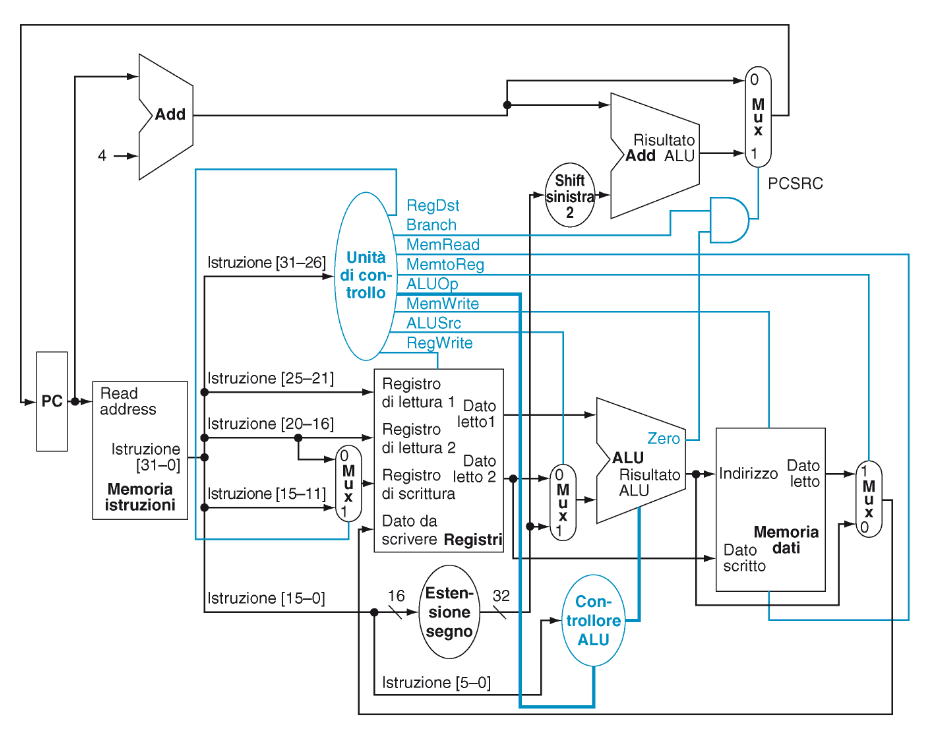
\includegraphics[scale=0.2]{Pictures/CPUComplessiva.png}
  \caption{Una CPU molto dettagliata}
  \label{fig:boat1}
\end{figure}
Si faccia riferimento alle slides per una spiegazione dei segnali di controllo. 
\subsubsection{Unit\`a di controllo}
\`E un'unit\`a funzionale combinatoria che prende come input il codice operativo dell'istruzione e genera i comandi del caso 
\subsubsection{Salto incondizionato}
In questa operazione il PC viene incrementato di 4, i suoi quattro bit significativi rimangono uguali, dal 27 al 2 sostituiti con il campo indirizzo dell'istruzione 
i due bit meno significativi settati a 0.
\section{Conclusione}
Le istruzioni raramente vengono concluse in un unico ciclo in quanto sono le pi\`u lente a dettarlo e non si riesce a fare ottimizzazioni aggressive sulle cose pi\`u 
frequenti.
